\newpage
\section{Theory}
\label{sec:theory}

The Multiply Accumulate Circuit contains two subsystems, as specified in the \autoref{tab:specifications}, a FSM and a MAC unit. In this section we are going to explain the functions of each subsystem and the principles used in circuit design. In \autoref{fig:blokk} the two subsystems are shown and how they connect to each other. There are five inputs, a clock signal, Run, Reset and two 2-bit inputs A and B. These will together determine what the 8-bit output Y will be. Between the Final State Machine and the MAC unit, some control signals are sent to make sure the MAC unit processes the data and makes the correct operations. 

\begin{figure}[H]
    \centering
    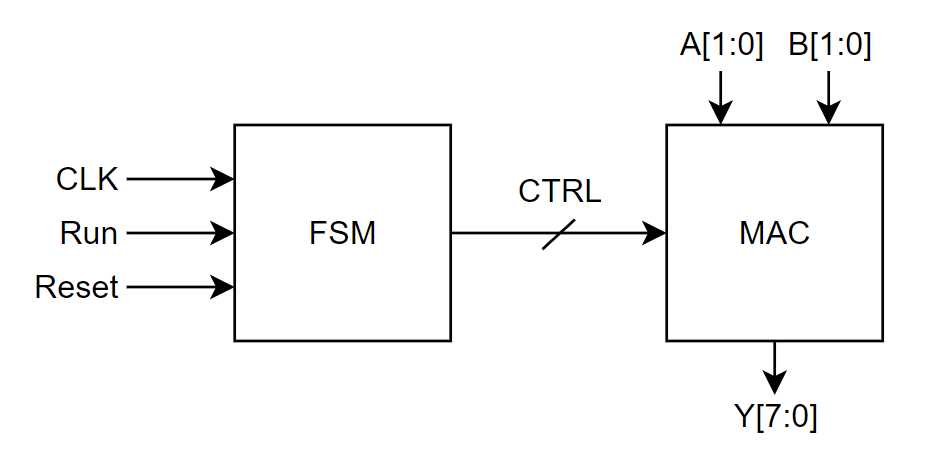
\includegraphics[width=0.7\textwidth]{Figures/Blokk.png}
    \caption{An overview of the complete system, with inputs CLK, Run, Reset, A[1:0] and B[1:0], and output Y [7:0].}
    \label{fig:blokk}
\end{figure}

\subsection{Finite State Machine}
\label{subsec:fsm_theory}

A finite state machine (FSM) is a model used to describe a system with a finite number of states. It operates by transitioning from one state to another in response to inputs, following a defined set of rules. FSMs consist of:

\begin{enumerate}
    \item \textbf{States}: These represent distinct configurations that the system can be in.
    
    \item \textbf{Transitions}: These are directed connections between states, triggered by specific input conditions. Transitions determine the movement from one state to another.
    
    \item \textbf{Inputs}: These are external signals that trigger state transitions. Inputs influence the behavior of the FSM.
    
    \item \textbf{Outputs}: FSMs may generate outputs in response to inputs and state transitions. Outputs convey information about the current state or operation of the system.
\end{enumerate}

\noindent
FSMs can be classified into two main types:

\begin{enumerate}
    \item \textbf{Mealy Machine}: In a Mealy machine, the output depends on both the current state and the input. The output is produced immediately after an input is received or a state transition occurs. 
    
    \item \textbf{Moore Machine}: In a Moore machine, the outputs depend only on the current state. The output is associated with the state itself, so it changes only after a state transition.
\end{enumerate}

\noindent
Generalized circuit diagrams for Moore and Mealy FSMs are shown in figure~\ref{fig:general_fsm}.

\begin{figure}[H]
    \centering
    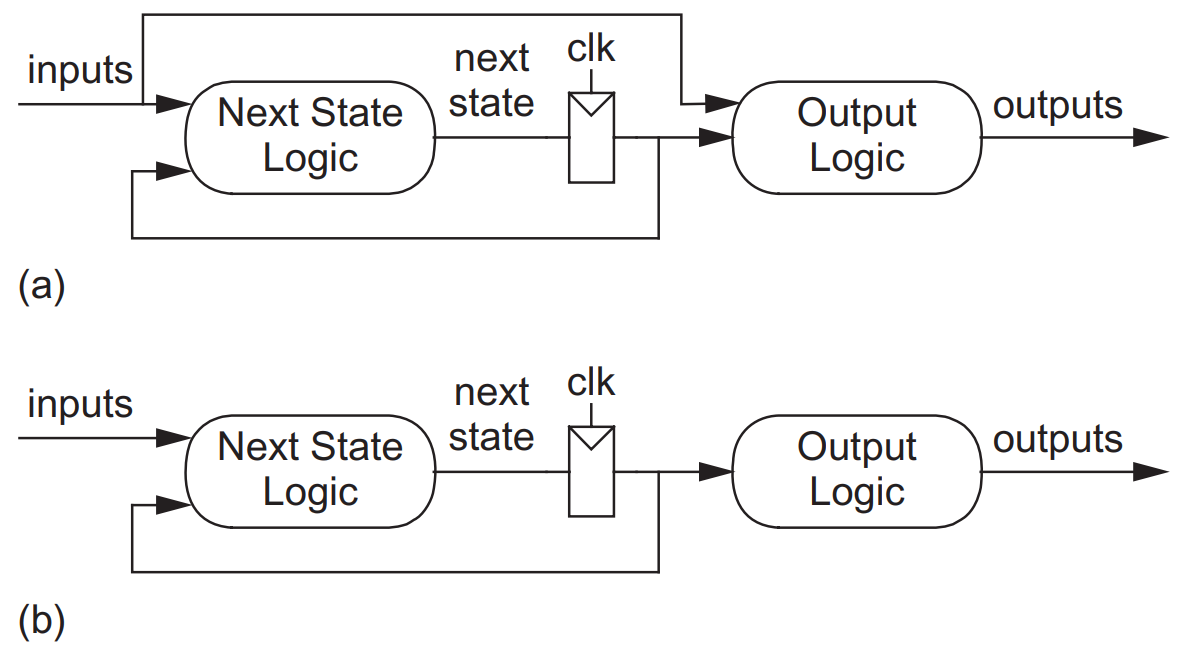
\includegraphics[width=0.8\textwidth]{Figures/general fsm diagrams.png}
    \caption{a: Mealy FSM. b: Moore FSM. (Figure is taken from \cite[p.735]{CMOS_VLSI_design})}
    \label{fig:general_fsm}
\end{figure}


\noindent
A certain design procedure can be used for the design of FSMs~\cite{digital_design}:

\begin{enumerate}
  \item From the word description and specifications of the desired operation, derive a state diagram for the circuit.
  \item Reduce the number of states if necessary.
  \item Assign binary values to the states.
  \item Obtain a binary-coded state table.
  \item Choose the type of flip-flops to be used.
  \item Derive the simplified flip-flop input equations and output equations.
  \item Draw the logic diagram.
\end{enumerate}


\subsection{MAC}
\label{subsec:MAC_theory}

The MAC unit will, according to the specifications given in \autoref{tab:specifications}, receive two 2-bit inputs, A and B, which will be multiplied and added to C, as shown in \autoref{eq:mac}. 

\begin{equation}
    \label{eq:mac}
    C \leftarrow C + (A \cdot B)
\end{equation}

 This should happen every rising edge of the clock, as defined by specification 8 in \autoref{tab:specifications}. The MAC unit consist of a multiplier, an adder and an accumulator. The layout of the MAC is shown in \autoref{fig:mac-blokk}. 

\begin{figure}[htpb]
    \centering
    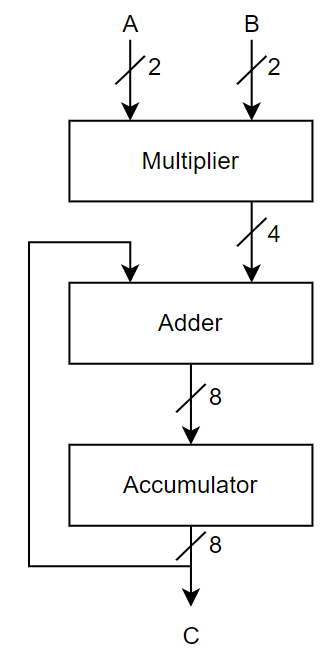
\includegraphics[width=0.3\textwidth]{Figures/mac-blokk.png}
    \caption{Layout of MAC unit, with inputs A[1:0] and B[1:0], and output C[7:0].}
    \label{fig:mac-blokk}
\end{figure}


\subsubsection{Multiplier}
The multiplier takes in A and B, two 2-bit inputs, and multiplies them. Since the inputs A and B are 2-bit inputs they are only able to represent values 0-3. This means that the highest possible output from the multiplier is 9, so that the output of the multiplier has to be at least 4-bit. 

\subsubsection{Adder}
As shown in \autoref{fig:mac-blokk}, the adder has to take the sum of a 4-bit number (A) and a 8-bit number (B). Since the multiplier only outputs a 4-bit number, the four most significant bits of A will always be zero. 

\subsubsection{Accumulator}
The accumulator is an 8-bit register with control signals, Set (S) and Reset (R). These control signals are received from the FSM. 

The registers can be made using latches. Latches store the value, but is not rising edge triggered. To create a edge triggered register, two latches can be connected in series with one master and one slave latch. The master and slave work on opposite clock inputs, and therefore create a edge triggered register. 

\begin{figure}[H]
    \centering
    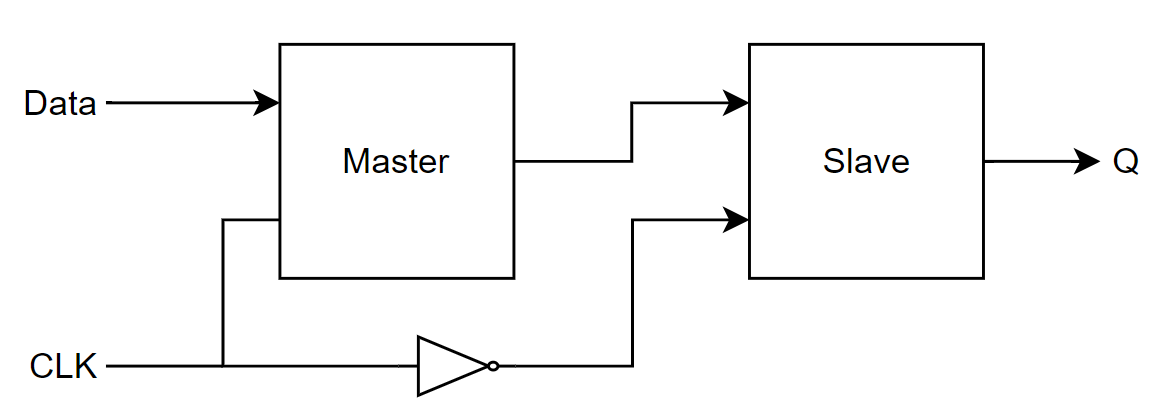
\includegraphics[width=0.9\textwidth]{Figures/DFF_Block.png}
    \caption{Relationship between master and slave latch in a D flip-flop.}
    \label{fig:enter-label}
\end{figure}

This type of register are called D flip-flops, which only change the stored value at the edge of the clock signal. These are used to achieve specification 8 in \autoref{tab:specifications}. The latches will in \autoref{sec:method} be designed to become rising edge triggered.

\subsection{Static Power Consumption}
\label{subsec:low_power}

One can consider many aspects of a circuit design to affect the static power consumption. Static power consumption in a circuit is primarily associated with leakage currents in transistors. The characteristics defined by a specific transistor technology as well as its width and length can influence the size of the leakage currents. As the transistor technology is given by \autoref{tab:specifications}, we may consider changing the width and length within the specifications to optimize for low leakage currents. 

\subsubsection{Leakage current}

In a transistor, there are three leakage currents that exist: subthreshold, gate, and
junction leakage currents. Out of these the subthreshold leakage current is in most cases the largest.\cite[p.49]{Analog_integrated} The equation for subthreshold leakage current is given by \autoref{eq:subthresholdcurrent}.\cite[p.42]{Analog_integrated}

\begin{equation}
    \label{eq:subthresholdcurrent}
    I_{D(sub-th)} \approx I_{D0}\left(\frac{W}{L}\right)e^{\left(\frac{qV_{eff}}{nkT}\right)}
\end{equation}

As we can see in \autoref{eq:subthresholdcurrent}, the width-to-length ratio is proportional to the subthreshold leakage current. Therefore a smaller width and larger length can optimize the leakage current in the circuit.

Since $V_{eff} < 0$ in subthreshold region the leakage current will have a proportional relationship with the temperature. So when the temperature increases, the leakage current will increase as well. 

In an ideal scenario, one might approximate to say that the leakage current increases linearly with the number of transistors, assuming each transistor contributes an equal amount to leakage current. However, in reality, the relationship is more complex. This simplification is useful nevertheless and is used when considering design choices in this project.

\subsubsection{Transistor Stacking}
Another way to decrease the leakage current is to use transistor stacking. When stacking transistors, like shown in \autoref{fig:transistor_stacking}, the voltage drop from $V_{DD}$ to $V_{SS}$, is split over both transistors. This makes the $V_{DS}$ for each transistor lower than if there was only one transistor. A lower $V_{DS}$ means a lower DIBL-effect, which in turn can result in a lower leakage current. This is explained in more detail in chapter 13.5.1 in \cite{transistor_stacking}.

\begin{figure}[H]
    \begin{minipage}{0.5\textwidth}
        \centering
        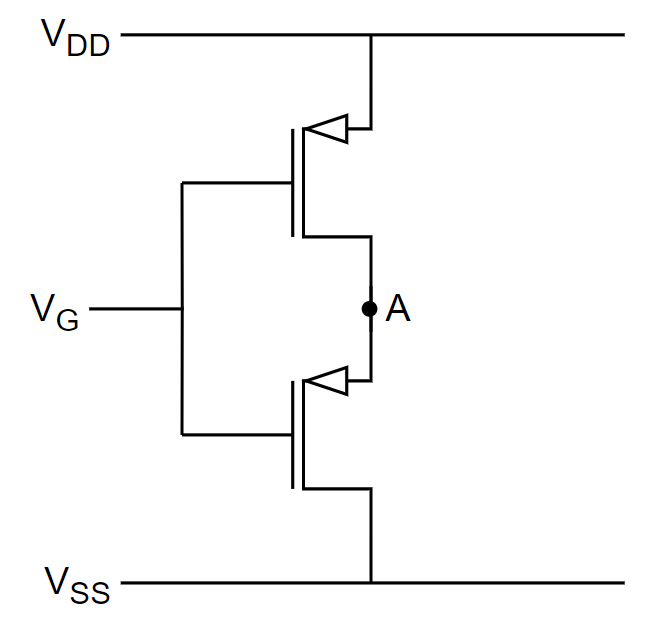
\includegraphics[width=\textwidth]{Figures/Transistor Stacking.png}
        \caption{\parbox{0.5\textwidth}{Transistor stacking with two transistors.}}
        \label{fig:transistor_stacking}
    \end{minipage}%
    \begin{minipage}{0.5\textwidth}
        \centering
        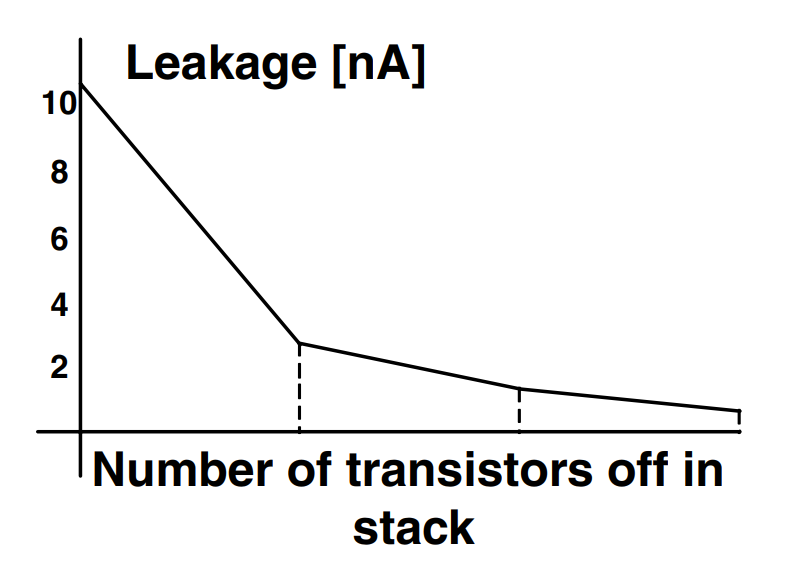
\includegraphics[width=\textwidth]{Figures/Leakage_current_ratios.png}
        \caption{\parbox{0.5\textwidth}{Leakage current with different number of transistor in stack. \cite[p.13-7]{transistor_stacking}}}
        \label{fig:leakage_current_ratio}
    \end{minipage}
\end{figure}

\subsubsection{Calculation of Static Power Consumption}
\label{subsubsec:SPC_Calc}
When calculating the static power consumption for the 1-bit register, we look at a state where the CLK is not running and the inputs, D, S and R, are set to low. The static power consumption is calculated by taking the leakage current in the $V_{DD}$ node and multiplying it with the voltage, as shown in \autoref{eq:power}. This shows that a lower supply voltage results in lower static power consumption.

\begin{equation}
    \label{eq:power}
    P = I_L \cdot V_{DD}
\end{equation}

\subsection{Static CMOS}\label{subsec:static_cmos}

The logic family used for this project is Static CMOS. This family provides strongly driven logic 1's and 0's, resulting in low static power consumption. The Static CMOS logic family is mainly identified by a PMOS pull-up network and a NMOS pull-down network as shown in \autoref{fig:static_CMOS}. These networks are put together in such a way that they drive the output in a mutually exclusive way, meaning that in a steady state there is no direct path between the supply voltage and ground. 

\begin{figure}[H]
    \centering
    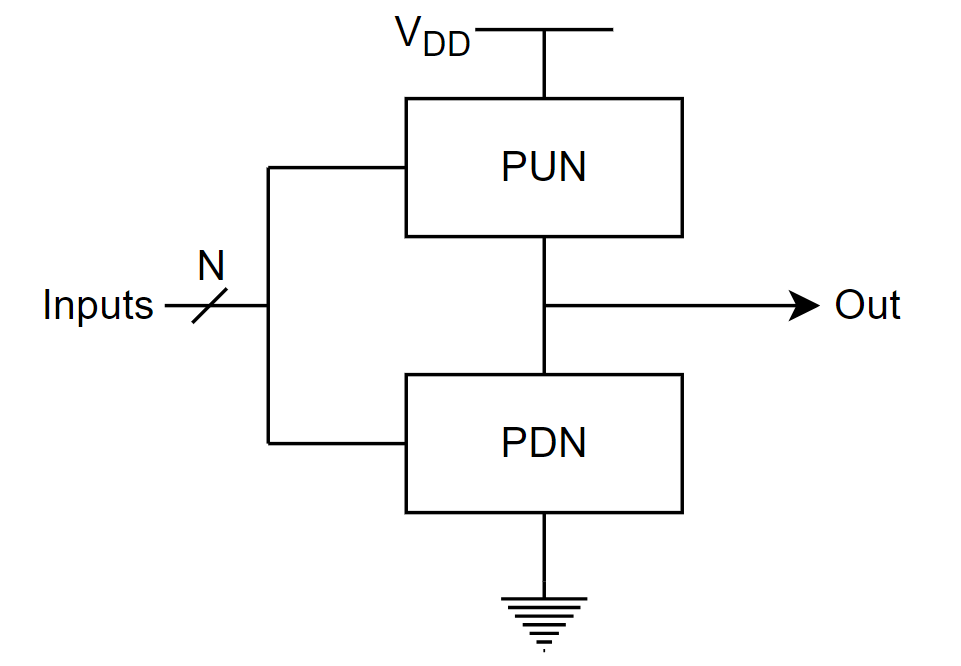
\includegraphics[width=0.6\textwidth]{Figures/Pull_UP_DOWN.png}
    \caption{General Static CMOS layout with Pull Up Network (PUN) and Pull Down Network (PDN).}
    \label{fig:static_CMOS}
\end{figure}


\subsection{Process Corners}
\label{subsec:corners}

Transistors may vary in design and therefore have different characteristics. In CMOS, there are two types of transistors with close to independent characteristics. We define these combinations of variations in the transistors as process corners. The variations are shown in \autoref{fig:cornersPlot}, where the first letter is the characteristics of the NMOS and the second is PMOS. 

\begin{figure}[H]
    \centering
    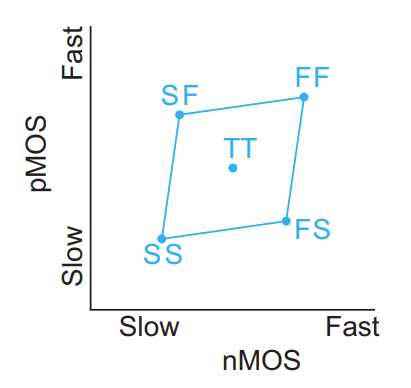
\includegraphics{Figures/CornersTheory.png}
    \caption{Process corners in a NMOS/PMOS plot \cite[p.245]{CMOS_VLSI_design}}
    \label{fig:cornersPlot}
\end{figure}

Often the different corners relate to different properties, as a fast PMOS may work under a higher frequency than a slow PMOS. A typical process corner is the nominal process corner and often represent the average characteristics of a transistor, with a balance between speed and power consumption. The fast corner gives a transistor that can handle a higher frequency, but in return has a higher power consumption and often is more susceptible to noise and variations in the environment. As for the slow process corner, the opposite is true as it prioritizes low power consumption while sacrificing speed.

It's important to take the different corners into consideration when designing a integrated circuit, as these process corners may be incorporated in the circuit during the manufacturing process. 
